\section{Agent Notion}

All agent-oriented software is based on the notion of agent defined in \cite{DUMMY:1}. \par
\theoremstyle{definition}
\begin{definition}{Agent}
    -- computer system that is situated in some environment, and that is capable of autonomous action in this environment in order to meet its delegated objectives.
\end{definition}
After disassembling this definition the list of characteristics that are required by each agent can be created. However, most people use the term ``agent'' when talking about the entity with a bit broader list of characteristics, also known as ``intelligent agent'' \cite{DUMMY:6}. Main characteristics of intelligent agent are:
\begin{itemize}
 \item \textbf{Autonomy}, usually perceived as an ability to operate without direct intervention as well as control over the internal state.
 \item \textbf{Social ability} -- an ability to interact with other agents, usually essential to achieve the goal.
 \item \textbf{Reactivity} -- an ability to receive information from their environment and respond to that information.
 \item \textbf{Proactiveness} -- goal-driven behaviour.
\end{itemize}
In \cite{dummy:1} the multi-agent system is defined as the one that consists of agents, but due to questionable restrictions the definition in this book is a bit different.
\begin{definition}{Multi-agent system}
is any system that includes more than one agent.
\end{definition}
Agents are often being disassembled into 3 parts: perception (receiving and preprocessing the input), decision-making and effectors (responsible for influencing the environment). The structure is shown in Figure \ref{GnomeAgent}. Agents constantly receive information from the environment, process it, then use it to choose the information (depicted as "actions" arrow) they are going to send to the environment. Effectors and sensors are used to formalize and restrain the data that can be passed to and from the environment. \par
    \begin{figure}[h!]
     \begin{center}
      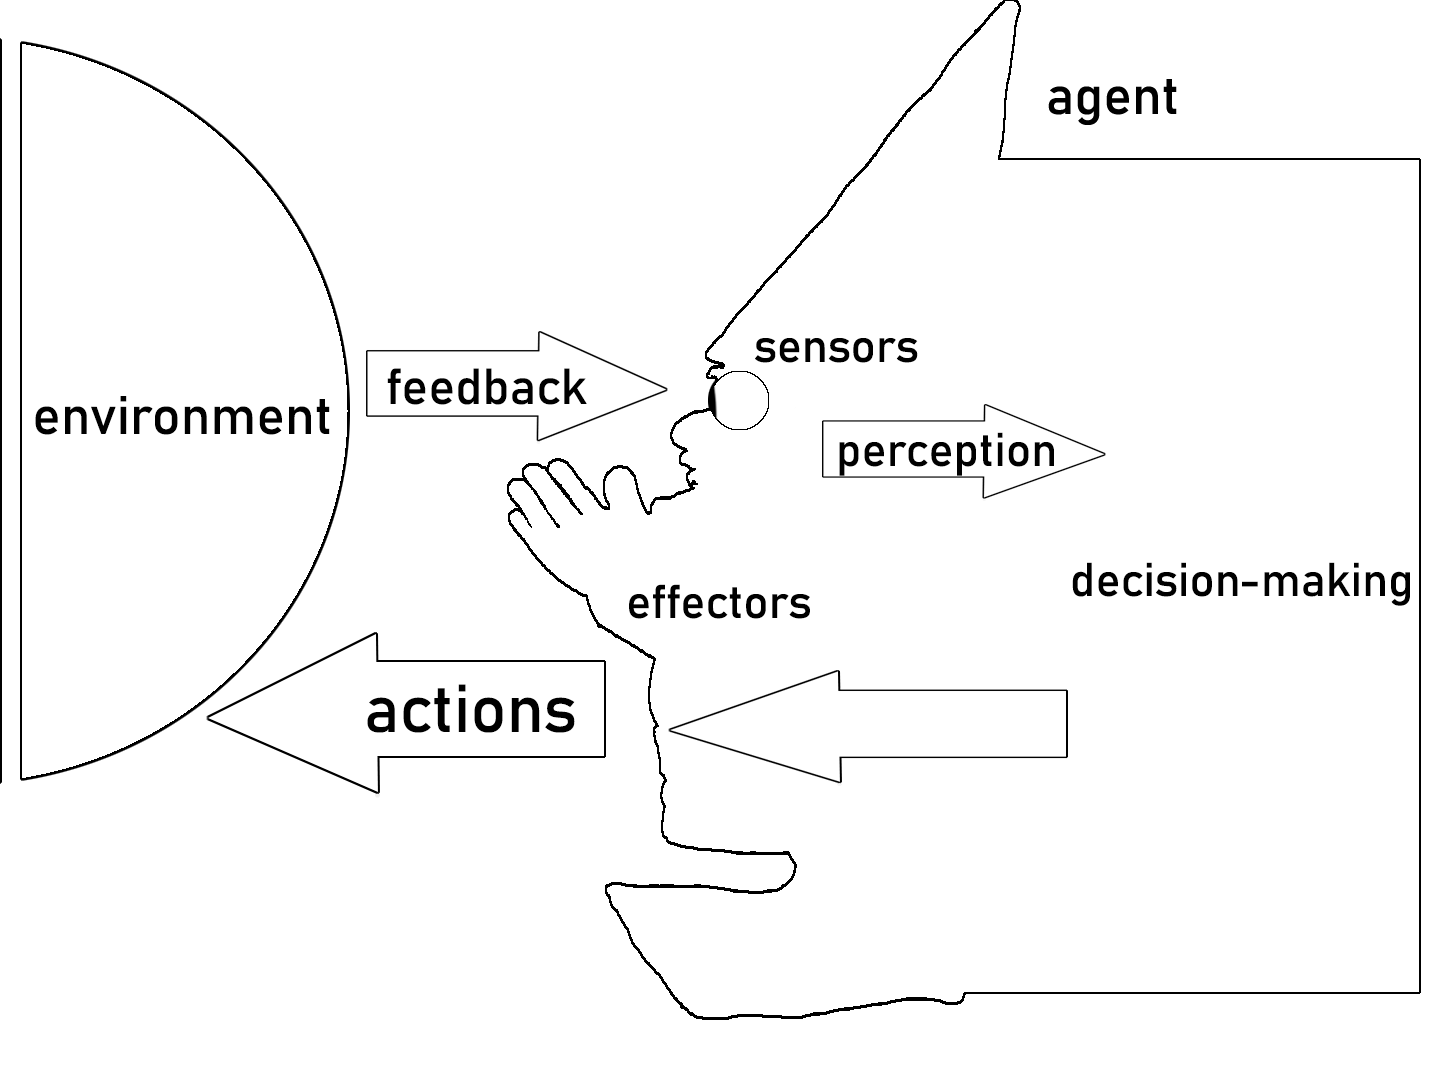
\includegraphics[width=400pt]{gnome_agent}
      \caption{Gnome agent}
      \label{GnomeAgent}
      \end{center}
    \end{figure}
%In classic multi-agent theory agents are being contained by their environment , therefore in any particular moment any agent can interact only with one environment (and, transitively, with other agents in this environment).

